\section[Piloto geométrico--topológico: PLL, MAVPD y Wu]
{Piloto dinámico geométrico--topológico: PLL, MAVPD y Wu}
\label{sec:resultados-piloto-gt}

La campaña B0--B2 de \cref{sec:campana-gt} integró el PLL lead--lag y el
MAVPD con \(q=1\), y el Chua arctangente de Wu con \(q=0.99\). El banco de
24 semillas produjo 90 trayectorias y 12 evaluaciones de borde al combinar
presupuestos y solucionadores. Todas las integraciones finalizaron sin fallos
numéricos.

El experimento compara semillas construidas con información geométrica y
semillas obtenidas por función descriptiva. Estudiamos qué destino alcanza
cada una y qué rasgos de esa respuesta se conservan al cambiar el integrador
y el presupuesto. Sus horizontes normalizados difieren de los usados para
localizar los ciclos de referencia.

La semilla \(p_+\) del PLL converge al foco con acuerdo entre métodos y
horizontes. En MAVPD, los PP alcanzan los ciclos interiores y las semillas
armónicas alcanzan el exterior, aunque algunos observables todavía varían
al ampliar la integración. En Wu, las respuestas permanecen acotadas durante
el intervalo estudiado, con discrepancias entre métodos. Estos desenlaces
determinan qué segmentos permiten explorar una frontera de cuenca.

\begin{hafocommonfigure}
\begin{center}
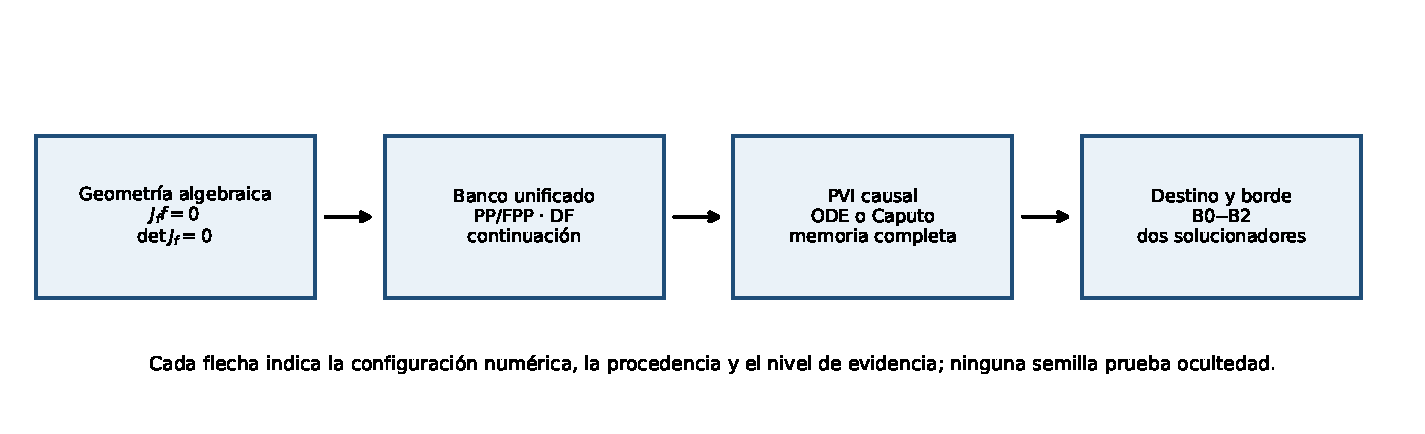
\includegraphics[width=0.96\linewidth]{figures/geometric_topological_pilot/00_ruta_geometrico_topologica.pdf}

\smallskip
\small\textbf{Ruta conceptual del piloto.} Relación entre álgebra, semillas,
transporte causal, clasificación y exploración de fronteras.
\end{center}
\end{hafocommonfigure}

\subsection{De los presupuestos normalizados a tiempos físicos}
\label{subsec:pilot-tau-star}

La tabla B0--B2 de la \cref{camp:tab-budgets} está expresada en las variables
adimensionales
\begin{equation}
 \widehat h=\frac{h}{\tau_*},\qquad
 \widehat T=\frac{T}{\tau_*},
 \qquad
 h=\widehat h\,\tau_*,\quad T=\widehat T\,\tau_*.
 \label{pilot:eq-budget-dimensionalization}
\end{equation}
La escala $\tau_*$ se fijó antes de clasificar destinos. Sea
$S=\operatorname{diag}(s_1,\ldots,s_n)$ la escala declarada del estado y
\begin{equation}
 \lVert v\rVert_S=\lVert S^{-1}v\rVert_2.
 \label{pilot:eq-scaled-norm}
\end{equation}
Para cada equilibrio $E$ se calculó el espectro de $J_E=DF(E)$. Como los
autovalores de una ecuación de Caputo de orden $q$ tienen dimensión
$\mathrm{tiempo}^{-q}$, la escala espectral coherente es
\begin{equation}
 \tau_{\mathrm{esp}}
 =\left(
   \max_{E}\max_{\lambda\in\sigma(J_E),\ \lambda\ne0}|\lambda|
  \right)^{-1/q}.
 \label{pilot:eq-tau-spectral}
\end{equation}
Para $q=1$ ésta es el inverso de la tasa espectral máxima. Como control de una
escala oscilatoria se usó, sobre la rama principal de $\lambda^{1/q}$,
\begin{equation}
 \tau_{\mathrm{osc}}
 =\min_{\Im(\lambda^{1/q})\ne0}
   \frac{2\pi}{|\Im(\lambda^{1/q})|}.
 \label{pilot:eq-tau-oscillatory}
\end{equation}
En Caputo esta cantidad compara escalas del problema lineal; no identifica
un periodo del PVI no lineal. Si no hay modos oscilatorios, tomamos
$\tau_{\mathrm{osc}}=+\infty$ para que no determine el mínimo.

La tercera escala procede directamente de la expansión Picard--Caputo. Para
una condición de reinicio $X_0$,
\begin{equation}
 S^{-1}[X(t_0+h)-X_0]
 =\frac{h^q}{\Gamma(q+1)}S^{-1}F(X_0)+O(h^{2q}).
 \label{pilot:eq-scaled-picard-crossing}
\end{equation}
Igualando a uno la norma del término principal se obtiene el tiempo de cruce
escalado
\begin{equation}
 \tau_{\mathrm{cr}}^{(q)}(X_0)
 =\left[
   \frac{\Gamma(q+1)}{\lVert F(X_0)\rVert_S}
  \right]^{1/q},
 \qquad
 \tau_{\mathrm{cr}}
 =\min_{X_0\in\mathcal S_{\mathrm{core}}}
   \tau_{\mathrm{cr}}^{(q)}(X_0).
 \label{pilot:eq-tau-crossing}
\end{equation}
Para una semilla estacionaria, $\lVert F(X_0)\rVert_S=0$, el tiempo de
cruce se interpreta como infinito. Finalmente fijamos, antes de clasificar
destinos,
\begin{equation}
 \tau_*=\min\{\tau_{\mathrm{esp}},\tau_{\mathrm{osc}},
                    \tau_{\mathrm{cr}}\}.
 \label{pilot:eq-tau-star}
\end{equation}

Los cálculos que activaron cada mínimo fueron los siguientes:
\begingroup
\footnotesize
\begin{longtable}{@{}L{2.0cm}C{2.25cm}C{2.25cm}C{2.25cm}L{4.4cm}@{}}
\caption{Derivación de $\tau_*$ para los tres casos.}
\label{pilot:tab-tau-star}\\
\toprule
Caso & $\tau_{\mathrm{esp}}$ & $\tau_{\mathrm{osc}}$ &
$\tau_{\mathrm{cr}}$ & Mínimo activo\\
\midrule
\endfirsthead
\toprule
Caso & $\tau_{\mathrm{esp}}$ & $\tau_{\mathrm{osc}}$ &
$\tau_{\mathrm{cr}}$ & Mínimo activo\\
\midrule
\endhead
PLL & $0.01369498063$ & $0.1550565455$ & $0.007324767204$ &
Cruce de $p_-$; $\lVert F(p_-)\rVert_S=136.5231102$.\\
MAVPD & $0.04262239251$ & $0.4812521201$ & $0.04702913869$ &
Espectral; $\max|\lambda|=23.46184579$.\\
Wu, $q=0.99$ & $0.2704709949$ & $2.295153098$ & $0.5755679794$ &
Espectral; $\max|\lambda|=3.649223883$ y el cruce se calculó sobre el banco
central FPP--A/FDF.\\
\bottomrule
\end{longtable}
\endgroup

En Wu, las semillas IDF transferidas y las condiciones ADM publicadas se
mantuvieron como controles externos al banco central que fijó la escala. El
protocolo permaneció fijado al incorporarlas. Si se incluye la
condición ADM de gran amplitud en el mínimo de
\eqref{pilot:eq-tau-crossing}, se obtiene $0.09700513591$; esta sensibilidad
muestra que la condición de gran amplitud introduce una escala más rápida.
La comparación realizada corresponde al banco central; ampliarlo requiere
recalcular la escala y comprobar de nuevo la resolución temporal.

Los presupuestos físicos efectivamente integrados fueron:
\begingroup
\tiny
\begin{longtable}{@{}L{1.8cm}C{0.7cm}C{2.05cm}C{2.15cm}C{2.15cm}C{1.8cm}C{1.1cm}@{}}
\caption{Paso, horizonte y descarte físico derivados de
\eqref{pilot:eq-budget-dimensionalization}.}
\label{pilot:tab-physical-budgets}\\
\toprule
Caso & Nivel & $\tau_*$ & $h$ & $T$ & $T_{\rm burn}$ & $N$\\
\midrule
\endfirsthead
\toprule
Caso & Nivel & $\tau_*$ & $h$ & $T$ & $T_{\rm burn}$ & $N$\\
\midrule
\endhead
PLL & B0 & $7.3247672\,10^{-3}$ & $1.46495344\,10^{-4}$ & $0.36623836$ & $0.18311918$ & 2500\\
PLL & B1 & $7.3247672\,10^{-3}$ & $7.3247672\,10^{-5}$ & $0.73247672$ & $0.36623836$ & 10000\\
PLL & B2 & $7.3247672\,10^{-3}$ & $3.6623836\,10^{-5}$ & $1.46495344$ & $0.878972064$ & 40000\\
MAVPD & B0 & $4.262239251\,10^{-2}$ & $8.524478502\,10^{-4}$ & $2.131119626$ & $1.065559813$ & 2500\\
MAVPD & B1 & $4.262239251\,10^{-2}$ & $4.262239251\,10^{-4}$ & $4.262239251$ & $2.131119626$ & 10000\\
MAVPD & B2 & $4.262239251\,10^{-2}$ & $2.131119626\,10^{-4}$ & $8.524478502$ & $5.114687101$ & 40000\\
Wu & B0 & $0.2704709949$ & $5.409419898\,10^{-3}$ & $13.52354975$ & $6.761774872$ & 2500\\
Wu & B1 & $0.2704709949$ & $2.704709949\,10^{-3}$ & $27.04709949$ & $13.52354975$ & 10000\\
Wu & B2 & $0.2704709949$ & $1.352354974\,10^{-3}$ & $54.09419898$ & $32.45651939$ & 40000\\
\bottomrule
\end{longtable}
\endgroup

En los dos casos enteros, DOP853 con
$(\mathrm{rtol},\mathrm{atol})=(10^{-10},10^{-12})$ fue el solucionador
principal y RK4 de paso fijo $h/2$ fue el control independiente. En Wu se
compararon ABM--PECE y EFORK--3 nativos, ambos desde $t_0=0$, con la misma
condición de reinicio y memoria completa; no hubo truncamiento de memoria ni
retroceso de terminal inferior.

\subsection{Álgebra de los PP enteros y de la semilla FPP--A}
\label{subsec:pilot-pp-algebra}

Para una ODE autónoma $\dot X=F(X)$,
\begin{equation}
 \ddot X=DF(X)\dot X=J(X)F(X)=A(X).
 \label{pilot:eq-integer-acceleration}
\end{equation}
Un punto perpetuo entero satisface $A(p)=0$ y $F(p)\ne0$. La segunda condición
es esencial: un equilibrio también anula $JF$, pero no es un PP.

\subsubsection{PLL en el cilindro}

Con $T=\tau_1+\tau_2$, el campo del PLL de \eqref{int:eq:pll} puede escribirse
en sus coordenadas físicas como
\begin{equation}
 F_x=\frac{-x+(\tau_1/2)\sin\theta}{T},\qquad
 F_\theta=\omega_\Delta-\frac{L}{T}x
 -\frac{L\tau_2}{2T}\sin\theta.
 \label{pilot:eq-pll-field}
\end{equation}
Al multiplicar por el Jacobiano,
\begin{equation}
 A_x=\frac{-F_x+(\tau_1/2)\cos\theta F_\theta}{T},
 \qquad
 A_\theta=-\frac{L}{T}
 \left[F_x+\frac{\tau_2}{2}\cos\theta F_\theta\right].
 \label{pilot:eq-pll-acceleration}
\end{equation}
Imponer \(A_x=A_\theta=0\) equivale a
\[
 F_x=\frac{\tau_1}{2}\cos\theta F_\theta,
 \qquad F_x=-\frac{\tau_2}{2}\cos\theta F_\theta.
\]
Igualar los lados derechos da \(T\cos\theta F_\theta/2=0\). Si
\(F_\theta=0\), ambas ecuaciones obligan a \(F_x=0\) y el punto es un
equilibrio. En un PP, por tanto, \(F_\theta\ne0\), \(\cos\theta=0\) y
\(F_x=0\). La misma condición se refleja en
\(\det J=L\cos\theta/(2T)=0\). Sustituyendo
$\theta=\pi/2,3\pi/2$ en $A=0$ se obtienen
\begin{equation}
 p_1=(\tau_1/2,\pi/2),\qquad
 p_2=(-\tau_1/2,3\pi/2),
 \label{pilot:eq-pll-pp-original}
\end{equation}
En esos puntos, \(F(p_1)=(0,\omega_\Delta-L/2)\) y
\(F(p_2)=(0,\omega_\Delta+L/2)\); son PP cuando la segunda componente
respectiva es distinta de cero. Sustituir \(F_x=0\) y \(\cos\theta=0\) en
\eqref{pilot:eq-pll-acceleration} anula exactamente ambos vectores \(A(p_i)\). En la carta usada para integrar,
$u=x-x_e$, $v=\theta-\theta_e$, con
$(x_e,\theta_e)=(0.01602944,0.7974826998815102)$, las semillas fueron
\begin{equation}
 p_+=(0.00637056,0.7733136269133863),\qquad
 p_-=(-0.03842944,3.914906280503180).
 \label{pilot:eq-pll-pp-shifted}
\end{equation}
No son un par por inversión central: para $\omega_\Delta\ne0$ la simetría
correcta es la cubierta $v\mapsto v+2\pi k$.

\subsubsection{MAVPD}

Para el campo
\begin{equation}
 F_1=\delta(\gamma u+v-u^3),\quad
 F_2=u-\xi v-w,\quad F_3=\rho v,
 \label{pilot:eq-mavpd-field}
\end{equation}
la multiplicación completa da
\begin{equation}
 A_1=\delta[(\gamma-3u^2)F_1+F_2],\quad
 A_2=F_1-\xi F_2-F_3,
 \quad A_3=\rho F_2.
 \label{pilot:eq-mavpd-acceleration}
\end{equation}
De $A_3=0$ sigue $F_2=0$. Entonces $A_2=0$ implica $F_1=F_3=\rho v$ y
$A_1=0$ se reduce a
$(\gamma-3u^2)F_1=0$. La rama $F_1=0$ es estacionaria; en la rama PP,
\begin{equation}
 u_*^2=\frac\gamma3,\qquad
 \delta\left(\frac{2\gamma u_*}{3}+v_*\right)=\rho v_*.
\end{equation}
Bajo \(\gamma>0\), \(\delta,\rho>0\) y \(\rho\ne\delta\), despejar la
segunda ecuación da \((\rho-\delta)v_*=2\delta\gamma u_*/3\). La condición
\(F_2=0\) da \(w_*=u_*-\xi v_*\). Por tanto,
\begin{equation}
 u_*=\pm\sqrt{\frac\gamma3},\qquad
 v_*=\frac{2\delta\gamma u_*}{3(\rho-\delta)},
 \qquad w_*=u_*-\xi v_*.
 \label{pilot:eq-mavpd-pp-derived}
\end{equation}
Con $(\gamma,\delta,\rho,\xi)=(0.1,100,200,3.1)$ resulta
\begin{equation}
 p_\pm=\pm(0.1825741858350554,
 0.01217161238900369,0.1448421874291439).
 \label{pilot:eq-mavpd-pp-numeric}
\end{equation}
El campo es impar, de modo que la inversión central relaciona exactamente las
dos trayectorias. El diagnóstico numérico del piloto produjo residuo impar
escalado cero, a la precisión almacenada, para DOP853 y RK4 en B2.

\subsubsection{Wu: raíces FPP--A y expansión de arranque}

Para el sistema de Wu de \cref{eq:chua_arctan,eq:parametros_wu}, sea
$h(x)=a_1x+a_2\arctan(\rho x)$. Con
\begin{equation}
 F_1=\alpha[y-x-h(x)],\quad F_2=x-y+z,\quad
 F_3=-\beta y-\gamma z,
\end{equation}
se obtiene, sin invocar una regla de cadena fraccionaria,
\begin{equation}
 A_1=\alpha[F_2-(1+h')F_1],\quad
 A_2=F_1-F_2+F_3,\quad A_3=-\beta F_2-\gamma F_3.
 \label{pilot:eq-wu-JF}
\end{equation}
El determinante se expande por la primera fila:
\[
 \det J=-\alpha(1+h')(\beta+\gamma)+\alpha\gamma
       =-\alpha[\beta+(\beta+\gamma)h'].
\]
En particular,
\begin{equation}
 \det J(x)=-\alpha\{\beta+(\beta+\gamma)h'(x)\}.
 \label{pilot:eq-wu-detJ}
\end{equation}
En una raíz no estacionaria de $JF=0$ el Jacobiano debe ser singular. Por ello
$p=h'(x_*)=-\beta/(\beta+\gamma)$ y
\begin{equation}
 x_*^2=\frac1{\rho^2}
 \left[
  \frac{a_2\rho}{-\beta/(\beta+\gamma)-a_1}-1
 \right].
 \label{pilot:eq-wu-xstar}
\end{equation}
Esta raíz requiere \(\rho\ne0\), \(p-a_1\ne0\) y un radicando no
negativo. Se obtiene al despejar
\(1+\rho^2x_*^2=a_2\rho/(p-a_1)\) en
\(h'(x_*)=a_1+a_2\rho/(1+\rho^2x_*^2)=p\).
Definiendo \(U=F_1\), las ecuaciones \(A_1=A_2=0\) dan
\(F_2=(1+p)U\), \(F_3=pU\). Las definiciones de \(F_1,F_2\) permiten
escribir
\[
 y_*=x_*+h(x_*)+U/\alpha,\qquad
 z_*=h(x_*)+(1+p)U+U/\alpha.
\]
Sustituirlas en \(F_3=-\beta y_*-\gamma z_*=pU\) produce
\[
 -\beta x_*-(\beta+\gamma)h(x_*)
 =\left[p+\gamma(1+p)+\frac{\beta+\gamma}{\alpha}\right]U.
\]
Si el coeficiente de \(U\) es distinto de cero, se obtiene
\begin{equation}
 U=-\frac{\beta x_*+(\beta+\gamma)h(x_*)}
 {\gamma+(1+\gamma)p+(\beta+\gamma)/\alpha},
 \quad
 y_*=x_*+h(x_*)+\frac U\alpha,
 \quad
 z_*=h(x_*)+(1+p)U+\frac U\alpha.
 \label{pilot:eq-wu-pp-solution}
\end{equation}
La evaluación de estas expresiones da el par
\begin{equation}
 \begin{aligned}
 p_\pm={}&\pm(0.3369817810952545,
 0.08157492826864399,\\
 &\hspace{3.3cm}-0.2549832342782551),\\
 \lVert F(p_\pm)\rVert={}&1.391241627161408,
 \end{aligned}
 \label{pilot:eq-wu-fppa-numeric}
\end{equation}
con residuo $\lVert J(p_\pm)F(p_\pm)\rVert$ y determinante numéricamente
nulos a 68 dígitos de precisión.

Para interpretar estas raíces en Caputo, supóngase \(F\in C^2\) cerca de
\(X_0\), con derivadas acotadas, y escríbase \(F_0=F(X_0)\),
\(J_0=DF(X_0)\). La forma de Volterra y el acotamiento local del campo dan
\(X(t_0+s)-X_0=O(s^q)\). La primera sustitución produce
\[
 X(t_0+s)-X_0=\frac{s^q}{\Gamma(q+1)}F_0+O(s^{2q}),
\]
y el desarrollo de Taylor del campo da
\[
 F(X(t_0+s))=F_0+
 \frac{s^q}{\Gamma(q+1)}J_0F_0+O(s^{2q}).
\]
Al integrar cada término contra el núcleo de Volterra,
\[
 \frac1{\Gamma(q)\Gamma(q+1)}
 \int_0^h(h-s)^{q-1}s^q\,\dd s
 =\frac{h^{2q}}{\Gamma(2q+1)},
\]
por la identidad beta de \cref{camp:eq-fractional-convolution}; el resto
\(O(s^{2q})\) integra a \(O(h^{3q})\). En consecuencia,
\begin{equation}
 X(t_0+h)=X_0+
 \frac{h^q}{\Gamma(q+1)}F_0+
 \frac{h^{2q}}{\Gamma(2q+1)}J_0F_0+O(h^{3q}).
 \label{pilot:eq-wu-picard-expansion}
\end{equation}
Por tanto $J_0F_0=0$ cancela el primer término de curvatura del arranque. El
conjunto espacial de raíces coincide con el conjunto PP de la ODE asociada y
es independiente de $q$; los pesos temporales y la evolución causal sí dependen
de $q$. Esta cancelación local se distingue de la aceleración fraccionaria
y de los eventos FPP--H dependientes de la historia.

\subsection{Criterios de comparación numérica}
\label{subsec:pilot-gates}

La primera condición fue que cada trayectoria permaneciera finita y dentro
del radio declarado. Para considerar estable la clasificación numérica de
una semilla exigimos simultáneamente:
\begin{enumerate}
 \item coincidencia del destino resuelto entre los dos solucionadores;
 \item error escalado en $0\le t\le10\tau_*$ no mayor que $10^{-3}$;
 \item diferencia relativa de observables no mayor que $5\%$;
 \item persistencia del destino y de los observables entre B1 y B2.
\end{enumerate}
Estas condiciones se evalúan por semilla: el buen acuerdo de una ruta no se
extiende a las demás. El estudio de una frontera añade sondeos de vecindad,
al menos tres segmentos iniciales no colineales con destinos diferentes y el
seguimiento de una trayectoria que permanezca entre ellos. El experimento
no completó esa construcción de frontera.

\subsection{Resultados del PLL: convergencia al foco y un transitorio}
\label{subsec:pilot-pll-results}

La semilla $p_+$ convergió al equilibrio conocido $E_{\rm focus}$ en B0, B1 y
B2 con ambos solucionadores. En B2, el error corto DOP853--RK4 fue
$2.16\,10^{-15}$, la diferencia de observables entre solucionadores fue
$1.12\,10^{-18}$ y la variación B1--B2 fue $2.48\,10^{-6}$.
La convergencia al foco se conserva en todas esas comparaciones.

La semilla $p_-$ permaneció acotada y ambos solucionadores concordaron
numéricamente hasta B2: el error corto bajó de $2.73\,10^{-10}$ en B0 a
$1.09\,10^{-12}$ en B2. Sin embargo, el destino permaneció transitorio y sin
resolución terminal. Ambos métodos aproximan una trayectoria semejante, pero
el intervalo observado no permite asignarle un destino. Las semillas del
ciclo y del separador también quedaron transitorias bajo los horizontes físicos
de esta normalización.

\ifHAFOBasinMaterial
El intervalo inicial de borde alrededor de
$(-0.0104934812033,-0.7974826998815)$ tenía extremos separados por
$2\,10^{-5}$ en $u$, es decir anchura cilíndrica escalada
$8.928571\,10^{-4}$. Como ambos extremos siguieron sin destino terminal en B1,
la bisección concluyó porque sus extremos no tenían destino resuelto; la
anchura permaneció sin cambios y la órbita de borde quedó pendiente.
\fi

\subsection{Resultados del MAVPD: los PP localizan ciclos interiores}
\label{subsec:pilot-mavpd-results}

Los dos PP tuvieron un resultado geométricamente informativo: $p_+$ alcanzó
la nube interna positiva y $p_-$ la nube interna negativa en B1 y B2, con
DOP853 y RK4.
Para $p_+$ en B2, el error corto fue $2.68\,10^{-14}$ y la diferencia entre
solucionadores en el mismo presupuesto fue $2.66\,10^{-6}$. No obstante, la
diferencia de observables B1--B2 fue $0.262445>0.05$; según el criterio
fijado, los observables todavía dependen del horizonte. Las semillas DF de la segunda
rama sí alcanzaron el ciclo exterior de referencia en B1--B2, pero su deriva de
horizonte fue $0.106908>0.05$. La separación entre destinos interiores y
exterior aparece con ambos métodos, mientras que la convergencia de los
observables requiere intervalos más largos.

Estos dos PP exactos se distinguen del banco de 96 condiciones perturbadas
estudiado en \cref{sec:correcciones-noviembre}. En ese banco, 91 respuestas
alcanzaron las ramas interiores y cinco permanecieron transitorias; ninguna
contactó la exterior. La comparación correspondiente de 96 semillas armónicas
produjo 48 destinos exteriores y 48 interiores. El resultado de los dos PP
centrales no implica que toda perturbación conserve su destino.

\ifHAFOBasinMaterial
El segmento de borde entre $p_+$ y la semilla DF exterior comenzó con anchura
escalada $1.450687592$. El primer punto medio fue clasificado como ciclo
exterior y redujo la anchura a $0.7253437961$. El segundo punto medio,
$(0.3081709798,0.05226056362,0.4511123215)$, cayó en el tercer destino, el ciclo
interior negativo de referencia. La bisección binaria se detuvo por la aparición
de ese tercer destino. Esto revela que el segmento no separa sólo dos
cuencas y motiva separar sus tres destinos antes de continuar el seguimiento
de borde. La aparición del tercer destino sobre un segmento no determina
por sí sola una frontera de Wada.
\fi

\subsection{Resultados de Wu: evaluación causal desde FPP--A}
\label{subsec:pilot-wu-results}

El banco Caputo comparó el par FPP--A con dos ramas de función descriptiva
fraccionaria, dos semillas obtenidas de la transferencia entera y las
condiciones iniciales ADM publicadas en \cite{Wu2023ArctanChua}. Todas las
corridas usaron $q=0.99$, $t_0=0$ y memoria completa. Las parejas por inversión
central FPP--A tuvieron residuo impar escalado exactamente cero, a la precisión
almacenada, con ABM y EFORK--3 en B0 y B2.

El resultado específico proveniente de puntos perpetuos fraccionarios es:
\begin{equation}
 p_\pm\xrightarrow[\text{ABM y EFORK--3}]{\mathrm{B0,B2}}
 \text{destino transitorio no resuelto},\qquad \text{trayectorias acotadas}.
 \label{pilot:eq-wu-fppa-destination}
\end{equation}
Para $p_+$, el error corto entre solucionadores fue $0.05360$, $0.05397$ y
$0.05420$ en B0, B1 y B2, respectivamente; todos exceden $10^{-3}$. Aunque la
variación de observables B1--B2 fue $0.01977$ para ABM y $0.04438$ para
EFORK--3, el destino no se resolvió. La anulación algebraica del término
$h^{2q}$ produce una propiedad local del arranque; en estas integraciones
no seleccionó una respuesta recurrente identificable en el horizonte probado.

Las semillas FDF2, IDF2 y ADM publicadas produjeron colas acotadas recurrentes,
pero en B2 ABM las clasificó en varios casos como periódicas sin identificar el
destino, mientras EFORK--3 las mantuvo como recurrentes sin identificarlo. La
discrepancia mantiene abierta la clasificación de esas respuestas. En este
experimento, una etiqueta periódica de Caputo
significa únicamente
\emph{casi periodicidad proyectada a tiempo finito}; no afirma la existencia de
una órbita periódica exacta.

\begingroup
\footnotesize
\begin{longtable}{@{}L{2.0cm}L{2.6cm}L{3.4cm}L{3.8cm}L{2.0cm}@{}}
\caption{Síntesis de destinos y criterios del primer piloto.}
\label{pilot:tab-results-summary}\\
\toprule
Caso & Ruta & Destino observado & Comparación decisiva & Resultado\\
\midrule
\endfirsthead
\toprule
Caso & Ruta & Destino observado & Comparación decisiva & Resultado\\
\midrule
\endhead
PLL & PP $p_+$ & Equilibrio $E_{\rm focus}$ & Destino y observables robustos B0--B2 & Convergente\\
PLL & PP $p_-$ & Transitorio acotado sin resolver & Falta destino terminal & Transitorio\\
\ifHAFOBasinMaterial
PLL & Segmento & Dos extremos sin resolver & Bisección sin iniciar & Borde sin resolver\\
\fi
MAVPD & PP $p_\pm$ & Ciclos interiores simétricos & Deriva B1--B2 de $26.24\%$ & Deriva temporal\\
MAVPD & DF exterior & Ciclo exterior de referencia & Deriva B1--B2 de $10.69\%$ & Deriva temporal\\
\ifHAFOBasinMaterial
MAVPD & Segmento & Aparece un tercer destino & Segmento no binario & Tres destinos\\
\fi
Wu & FPP--A $p_\pm$ & Transitorio acotado & Error corto ABM--EFORK $>10^{-3}$ & Desacuerdo numérico\\
Wu & FDF2, IDF2 y ADM & Recurrente o casi periódico proyectado & Desacuerdo de etiqueta en B2 & Destino sin resolver\\
\bottomrule
\end{longtable}
\endgroup

\subsection{Trayectorias y distribución de destinos}
\label{subsec:pilot-digital-figures}

\begin{hafobasinfigure}
\begin{center}
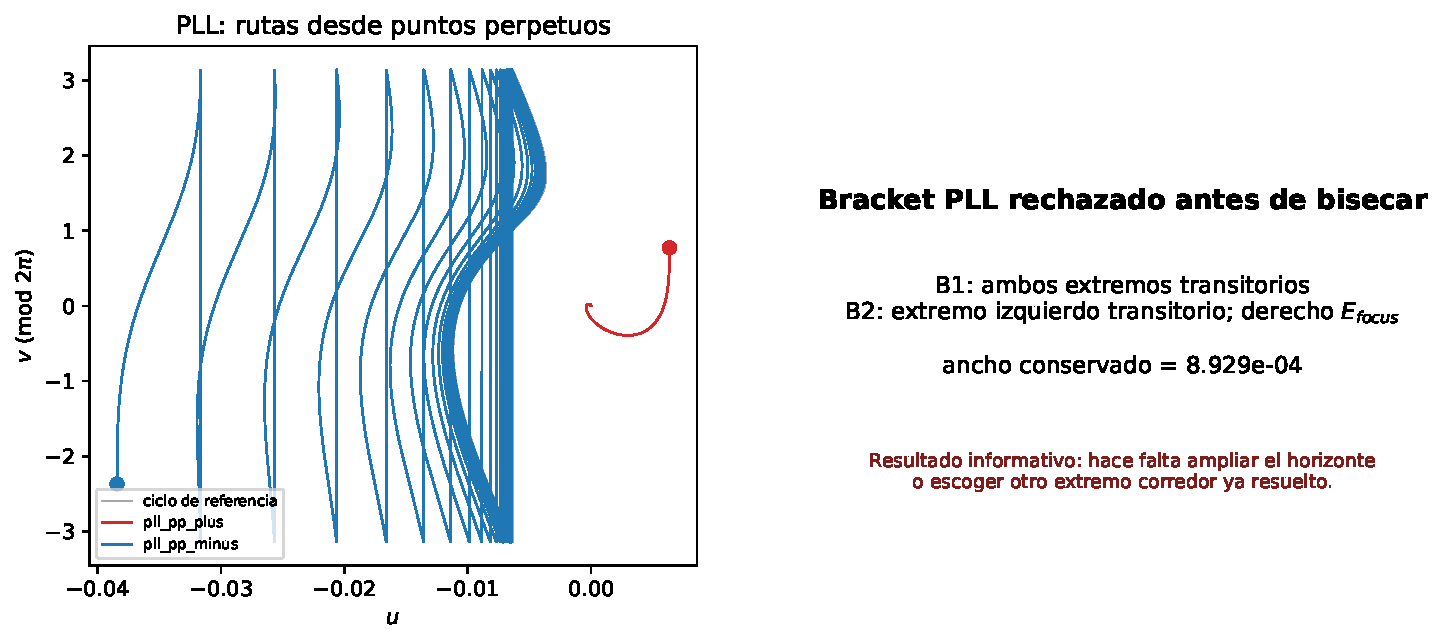
\includegraphics[width=0.96\linewidth]{figures/geometric_topological_pilot/01_pll_pp_y_borde.pdf}

\small\textbf{PLL.} Transporte de los PP e intervalo inicial. Los destinos y la
anchura corresponden al protocolo finito B0--B2.
\end{center}
\end{hafobasinfigure}

\begin{hafobasinfigure}
\begin{center}
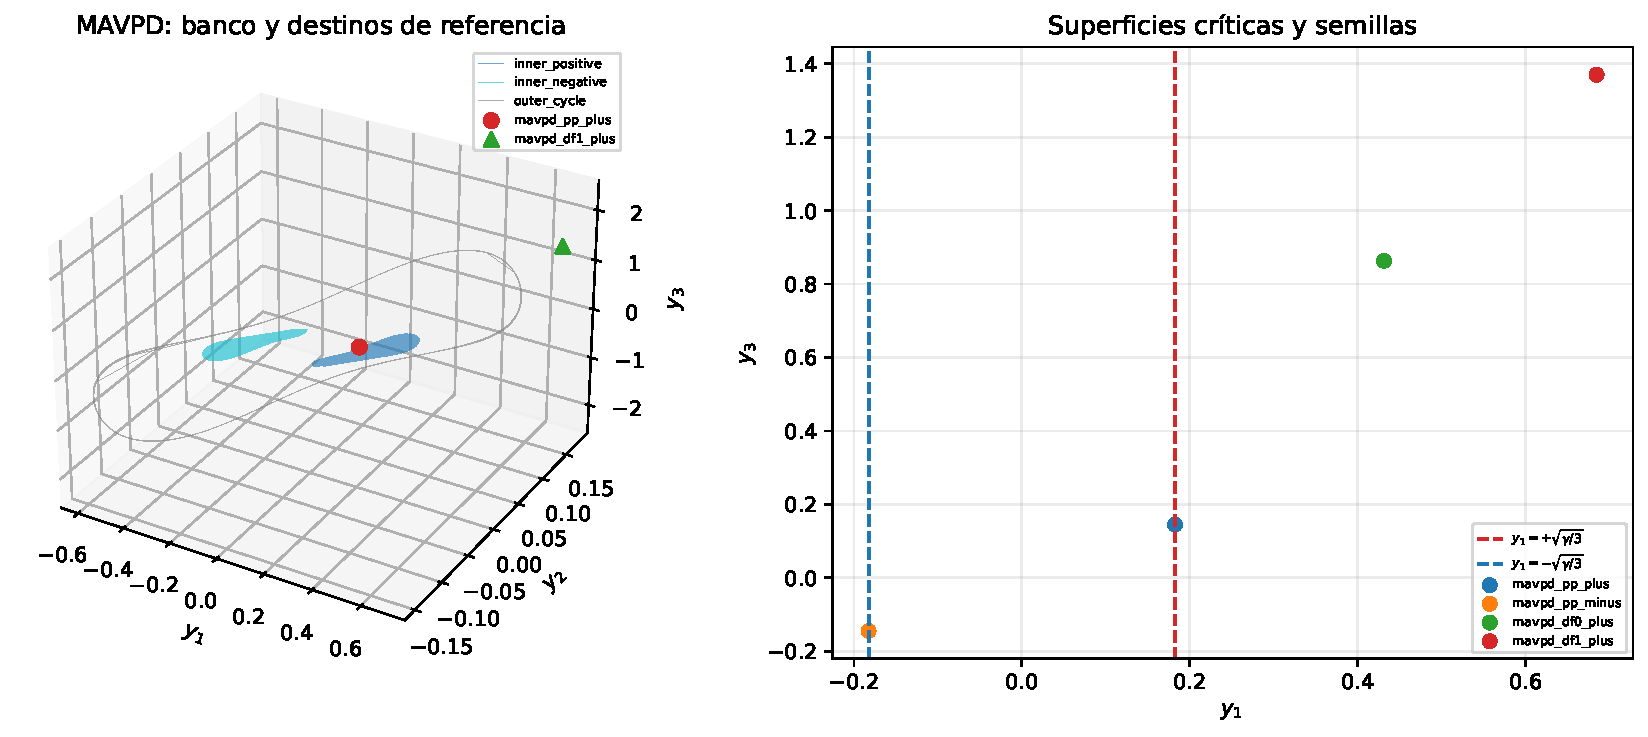
\includegraphics[width=0.96\linewidth]{figures/geometric_topological_pilot/02_mavpd_pp_superficie_destinos.pdf}

\small\textbf{MAVPD.} Superficie singular, PP, nubes de referencia y aparición
de un tercer destino sobre el segmento de borde.
\end{center}
\end{hafobasinfigure}

\begin{hafocommonfigure}
\begin{center}
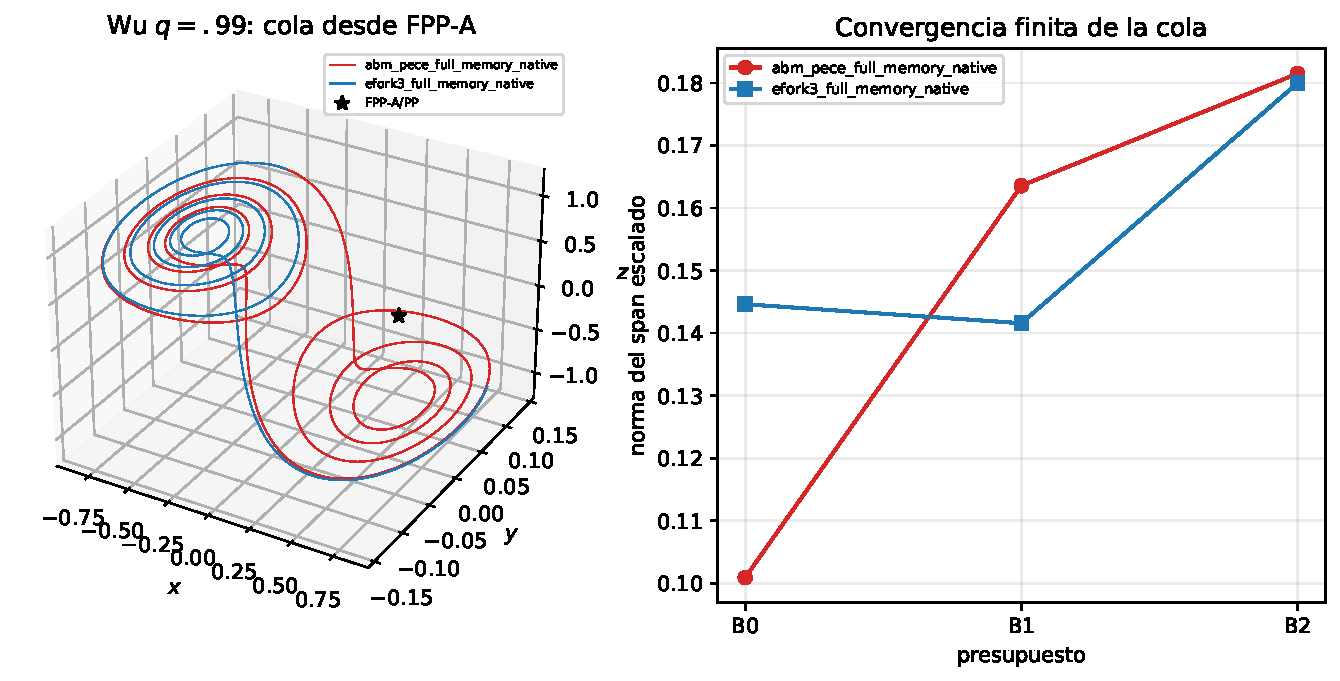
\includegraphics[width=0.96\linewidth]{figures/geometric_topological_pilot/03_wu_fpp_caputo_b0_b2.pdf}

\small\textbf{Wu, $q=0.99$.} Evolución causal con memoria completa desde el par
FPP--A. La comparación ABM--EFORK es finita y no certifica periodicidad.
\end{center}
\end{hafocommonfigure}

\begin{hafobasinfigure}
\begin{center}
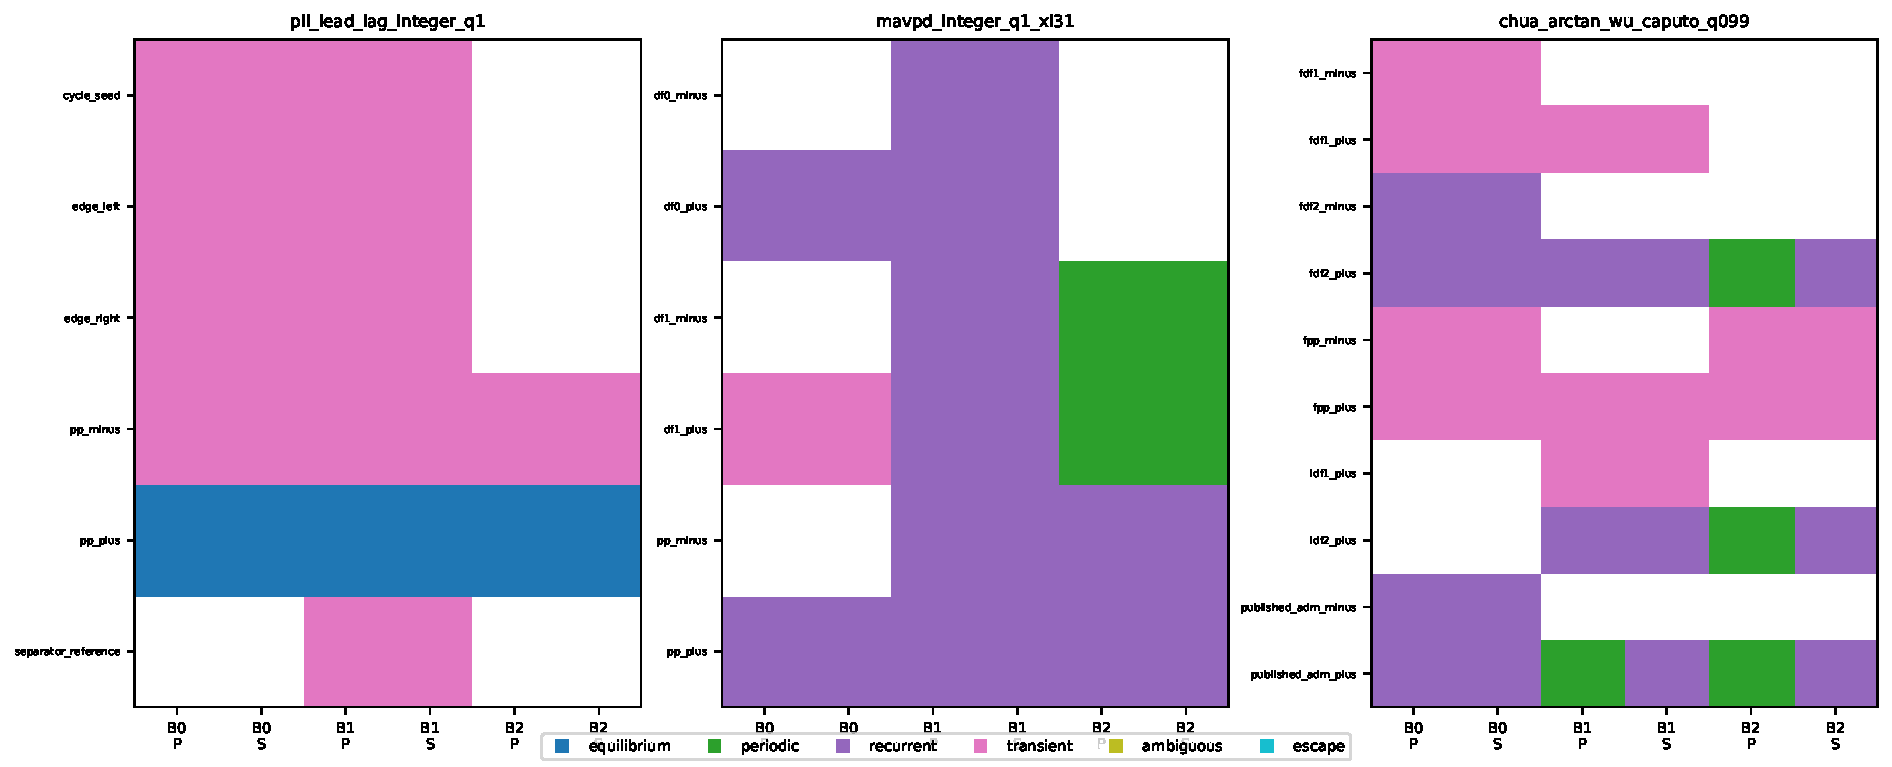
\includegraphics[width=0.96\linewidth]{figures/geometric_topological_pilot/04_matriz_destinos_b0_b2.pdf}

\small\textbf{Comparación entre semillas.} Etiquetas por semilla, presupuesto y
solucionador; una celda periódica de Caputo es sólo una etiqueta proyectada.
\end{center}
\end{hafobasinfigure}

\subsection{Antecedentes y alcance específico de la campaña}
\label{subsec:pilot-novelty}

\begin{longtable}{@{}L{3.2cm}L{4.1cm}L{5.8cm}@{}}
\caption{Antecedentes y evaluaciones realizadas en la campaña.}
\label{pilot:tab-novelty}\\
\toprule
Componente & Fundamento previo & Evaluación realizada en la campaña\\
\midrule
\endfirsthead
\toprule
Componente & Fundamento previo & Evaluación realizada en la campaña\\
\midrule
\endhead
PP entero & Definición $JF=0$, $F\ne0$, y uso como localizador
\cite{Prasad2015Perpetual,DudkowskiPrasadKapitaniak2017,
DudkowskiPrasadKapitaniak2018}. & Derivación y comparación homogénea con DF,
destinos de referencia y presupuestos B0--B2 en PLL y MAVPD.\\
Curvas y superficies & Superficies críticas y curvas conectantes
\cite{GilmoreEtAl2010Connecting,GuanXie2021Connecting}. & Integración de esas
semillas con un banco común de semillas y criterios de convergencia.\\
FPP--A & Volterra y expansión Picard de Caputo; ABM causal
\cite{DiethelmFordFreed2002}. & Cancelación del coeficiente $h^{2q}$ al imponer $JF=0$ y evaluación de las
raíces como semillas de reinicio.\\
Memoria & La dinámica Caputo requiere declarar terminal e historia
\cite{CongTuan2017Nonlocal,DoanKloeden2021Semidynamical}. & Comparación ABM y
EFORK--3 con el mismo $t_0$, reset y memoria completa, separada de las semillas
ADM publicadas.\\
Escala $\tau_*$ & Análisis dimensional y escalas espectrales estándar. & Regla
\eqref{pilot:eq-tau-star}, fijada antes de clasificar, para comparar los
presupuestos B0--B2 entre familias.\\
Comparación entre métodos & Diagnósticos numéricos y bisección de borde. &
Condiciones explícitas de concordancia para trayectorias, observables y
destinos, y separación de los segmentos con dos o tres respuestas.\\
\bottomrule
\end{longtable}

La expansión \eqref{pilot:eq-wu-picard-expansion} sustenta la selección de
semillas FPP--A. En Wu, las respuestas son acotadas, pero su clasificación
no converge todavía entre los dos integradores.

\subsection{Consecuencias para la localización}

Los tres casos muestran dificultades distintas. En PLL, un extremo sin
destino resuelto impide definir el par de cuencas que requiere una bisección.
En MAVPD, el obstáculo es la aparición de una tercera respuesta dentro del
segmento, aun cuando ambos extremos estén clasificados. En Wu, la diferencia
entre integradores precede al problema geométrico: la clasificación depende
de la aproximación numérica utilizada.

Un refinamiento $h,h/2,h/4$ sobre un intervalo físico común permite separar
el error de discretización de la deriva temporal de los observables. Con
destinos estables frente a esa comparación pueden construirse segmentos no
colineales, seguir una trayectoria de borde y formular un bloque aislante.
El índice de Conley requiere después imágenes exteriores y condiciones de
aislamiento, que no se deducen de una bisección inicial.
